% !TeX root = ../MAIN.tex
% !TeX encoding = UTF-8

\chapter{Anhang A - Benutzerdokumentation}
In diesem Kapitel wird die Benutzerdokumentation vorgestellt, die die Nutzung des Systems beschreibt und den Anwender bei der Verwendung der bereitgestellten Funktionen unterstützt.

\subsection{Stammdaten anlegen}
Für die Nutzung des NSP-Solvers müssen zunächst die erforderlichen Stammdaten im System angelegt werden. Voraussetzung dafür ist, dass das Angular-Frontend und das FastAPI-Backend gestartet sind und eine Verbindung zur Datenbank besteht. Anschließend können Daten wie die Mitarbeiter, die zu besetzenden Stationen sowie die benötigten Kompetenzen angelegt werden. Für jeden Mitarbeiter wird der Name, sowie die vorhandenen Kompetenzen hinterlegt. Anschließend werden die Stationen definiert, die im Dienstplan berücksichtigt werden sollen. Auch hier wird einfach ein Name und die erforderlichen Kompetenzen festgelegt. Außerdem müssen die Kompetenzen angelegt werden, damit diese den Mitarbeitern und Stationen zugeordnet werden können. Erst wenn alle erforderlichen Stammdaten vollständig erfasst wurden, können Schichtanforderungen definiert und Dienstpläne mithilfe des NSP-Solvers erstellt werden.
Abbildung \ref{fig:user_list} zeigt die Übersichts-Liste von Mitarbeitern.

\begin{figure}[h]
	\centering
	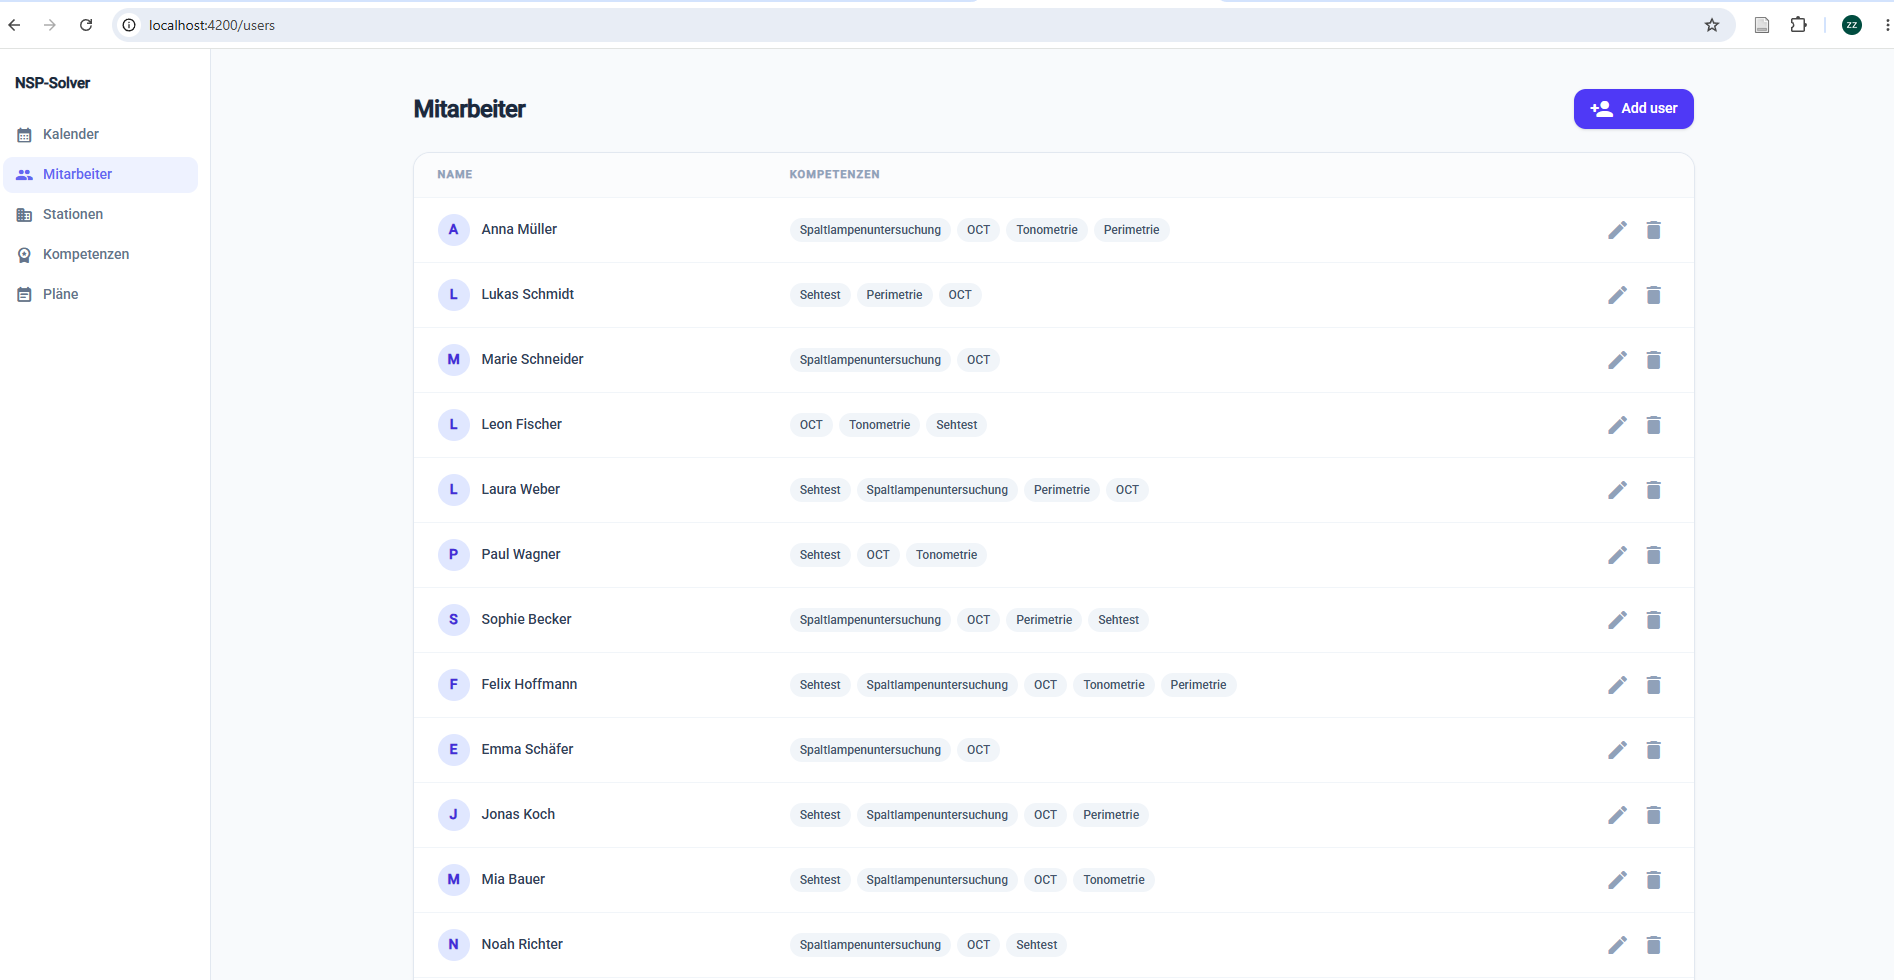
\includegraphics[width=\linewidth]{figures/user_list}
	\caption{
		Liste von Mitarbeitern
	}\label{fig:user_list}
\end{figure}

Über eine Unterseite kann man gewünschte Mitarbeiter mit den jeweiligen Kompetenzen anlegen. Die Unterseite wird in Abbildung \ref{fig:create_user} dargestellt.
\begin{figure}[h]
	\centering
	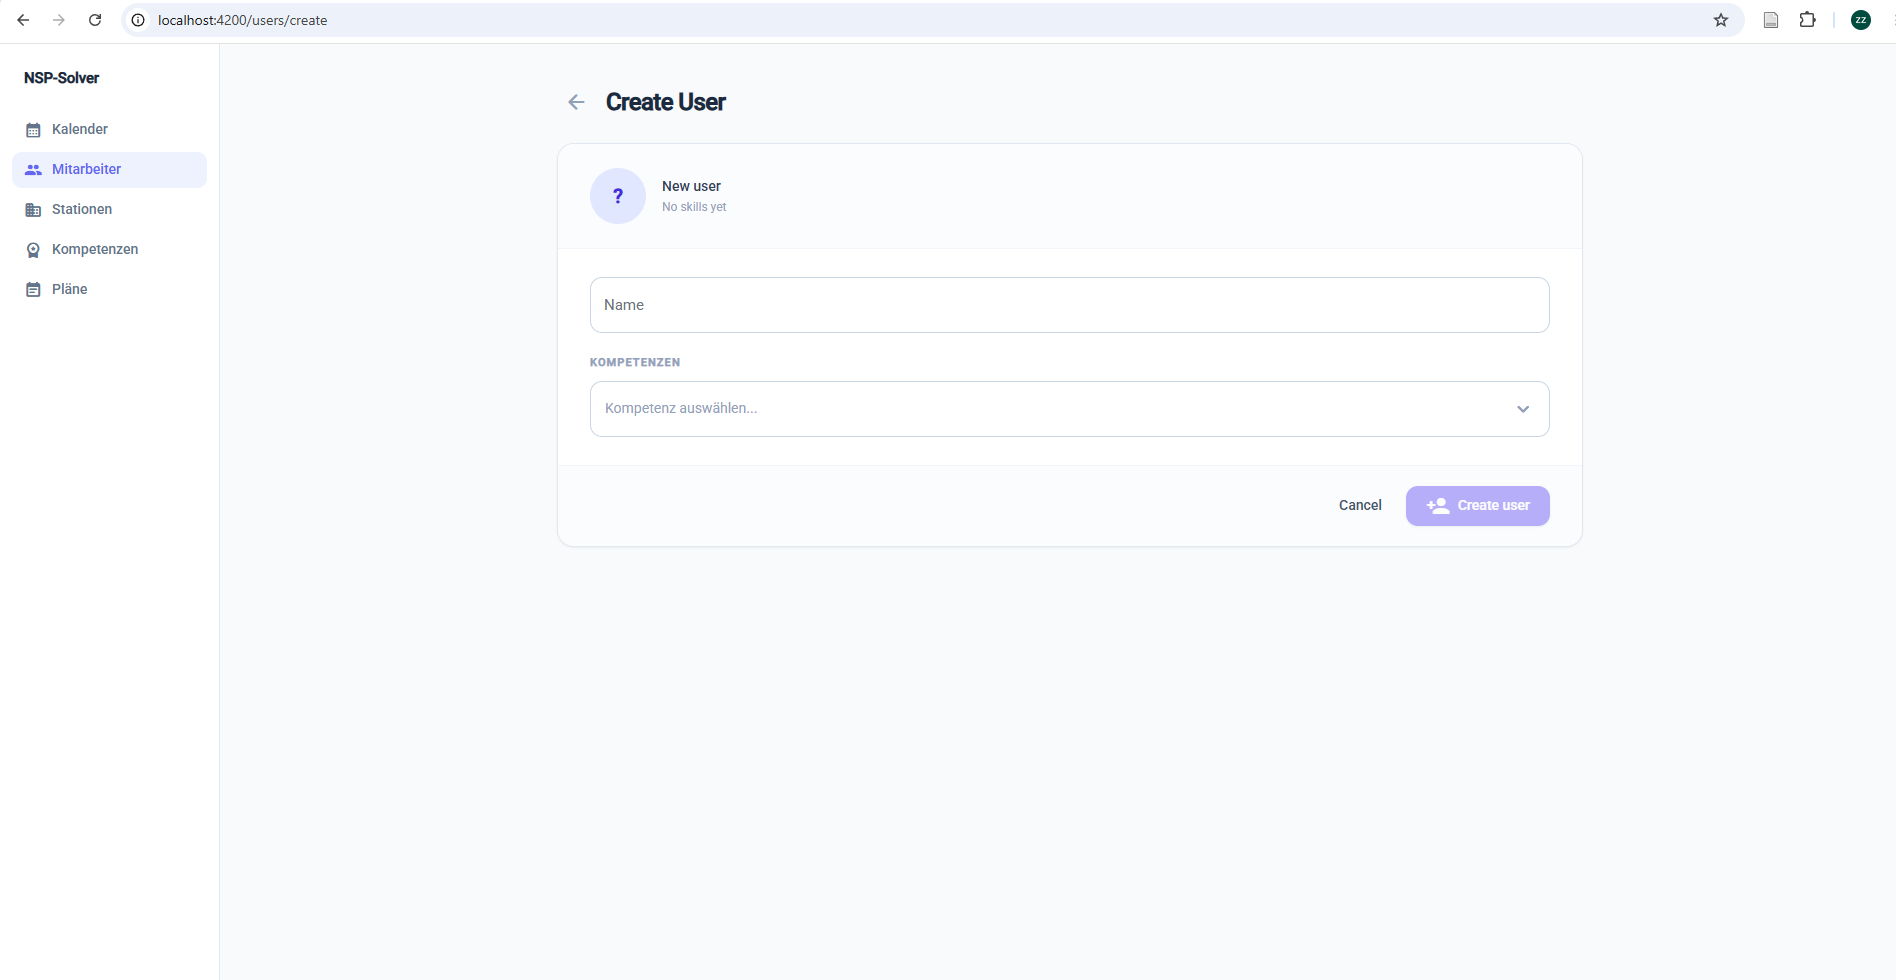
\includegraphics[width=\linewidth]{figures/create_user}
	\caption{
		Mitarbeiter erstellen
	}\label{fig:create_user}
\end{figure}

Analog dazu können auch Stationen und Kompetenzen auf den entsprechenden Unterseiten angelegt werden. \newline
Auf der Unterseite \textit{Kalendar} bekommt man eine Übersicht für den Monat. Wie die Unterseite aussieht, wird in Abbildung \ref{fig:calendar} dargestellt.

\begin{figure}[h]
	\centering
	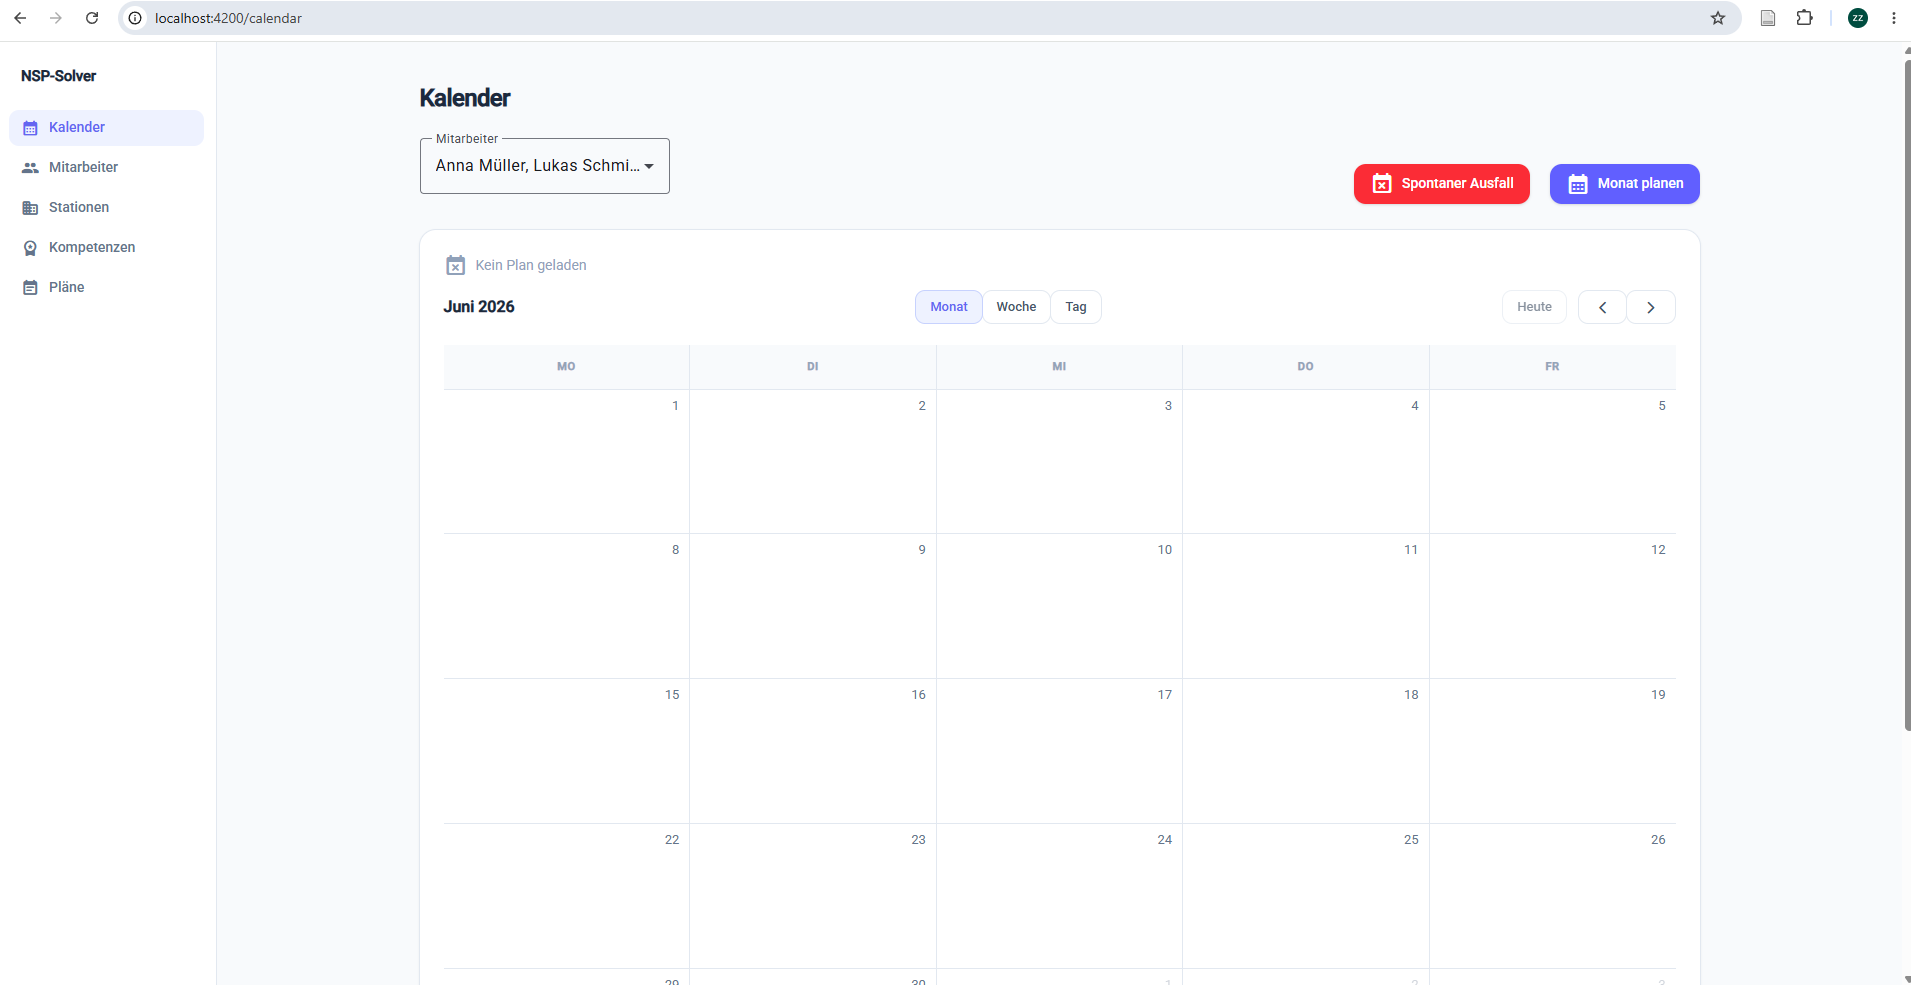
\includegraphics[width=\linewidth]{figures/calendar}
	\caption{
		Kalenderansicht
	}\label{fig:calendar}
\end{figure}

\subsection{(Re)-Scheduling}
Über den Button \textit{Monat planen} lassen sich vor dem Planungslauf individuelle Einschränkungen je Mitarbeiter festlegen. Das Dialogfenster ist in Abbildung \ref{fig:solver_dialog} dargestellt.  

\begin{figure}[h]
	\centering
	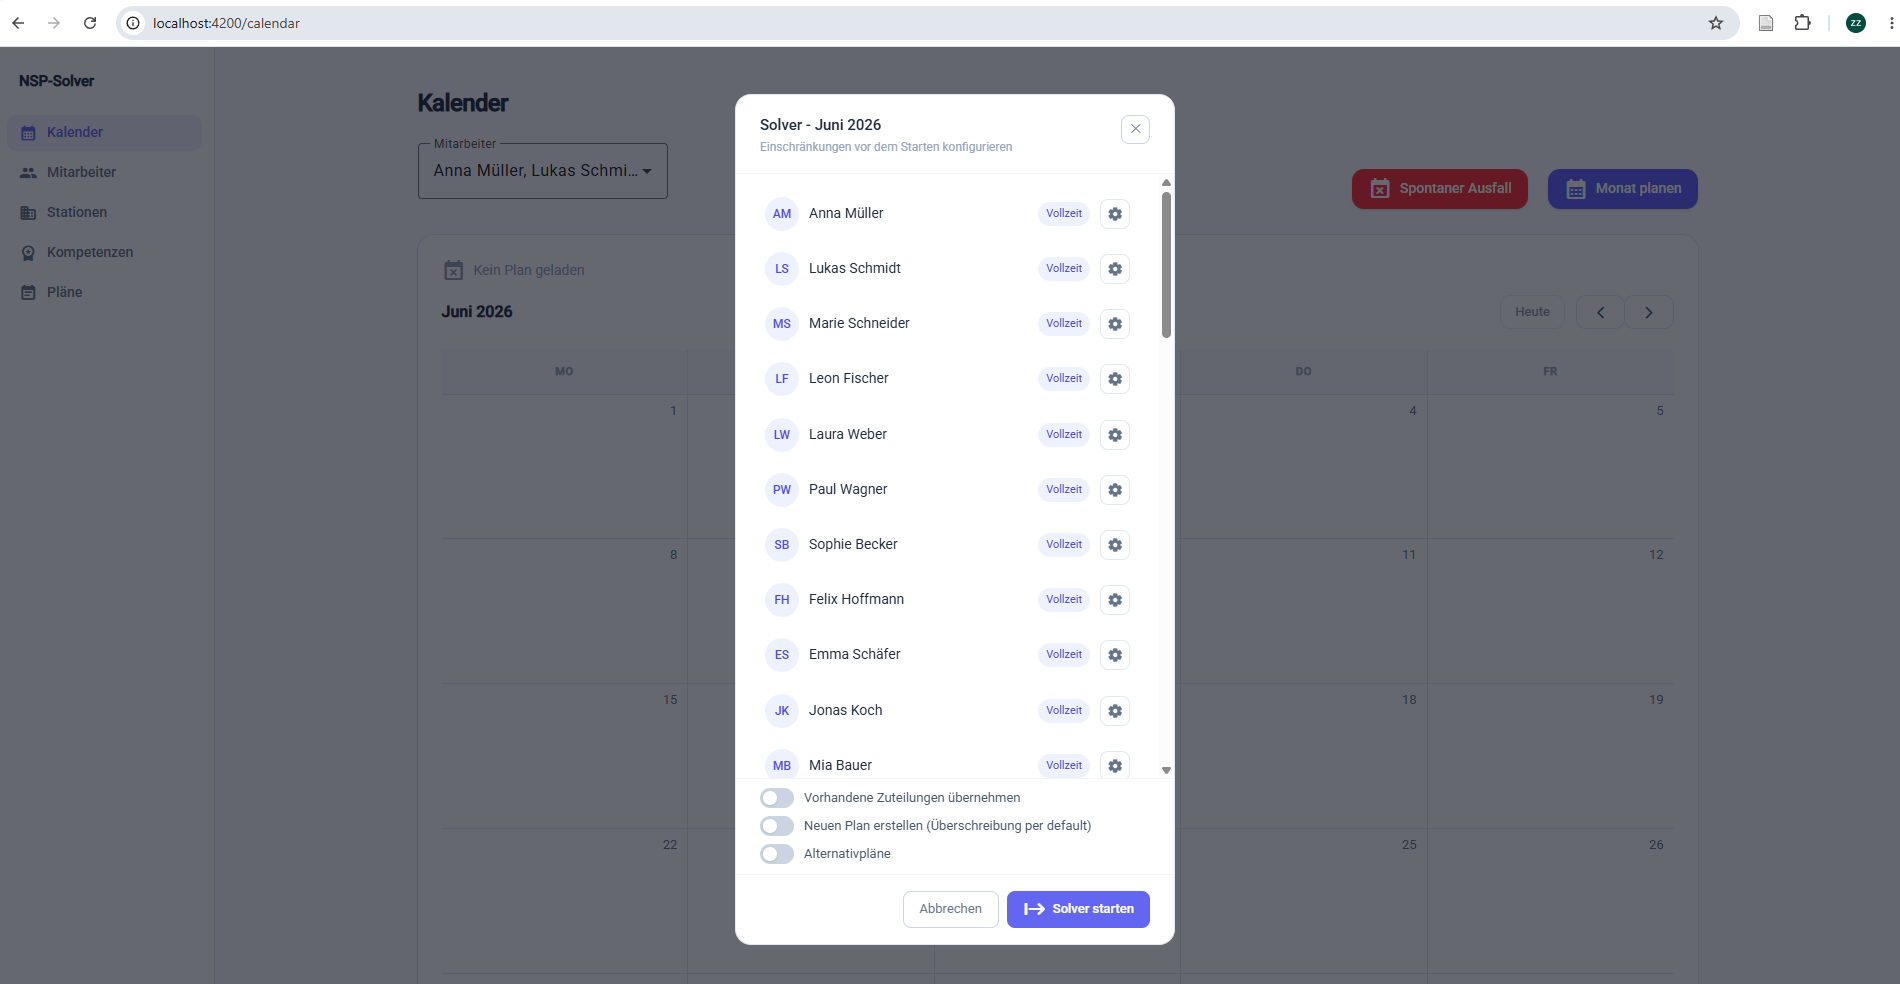
\includegraphics[width=\linewidth]{figures/solver_dialog}
	\caption{
		Solver-Dialogfenster
	}\label{fig:solver_dialog}
\end{figure}
Per Klick auf das Zahnrad-Symbol neben einem Mitarbeiter öffnet sich der Einschränkungsdialog, in dem die gewünschte Arbeitszeit für den Monat definiert wird, entweder als Vollzeit, als exakte Anzahl an Tagen oder als Spannweite. Im Abschnitt Verfügbarkeit kann anschließend über den Kalender angegeben werden, an welchen Tagen ein Mitarbeiter fix eingeplant werden soll oder nicht verfügbar ist. Nach dem Speichern der Einschränkungen stehen im Solver-Dialog außerdem drei Modi zur Auswahl: Vorhandene Zuteilungen übernehmen, Neuen Plan erstellen sowie Alternativpläne. Mit einem Klick auf \textit{Solver starten} wird die Planung unter Berücksichtigung aller konfigurierten Vorgaben ausgeführt. Das Dialogfenster für Einschränkungen wird in Abbildung \ref{fig:constraint_dialog} grafisch veranschaulicht.
\begin{figure}[h]
	\centering
	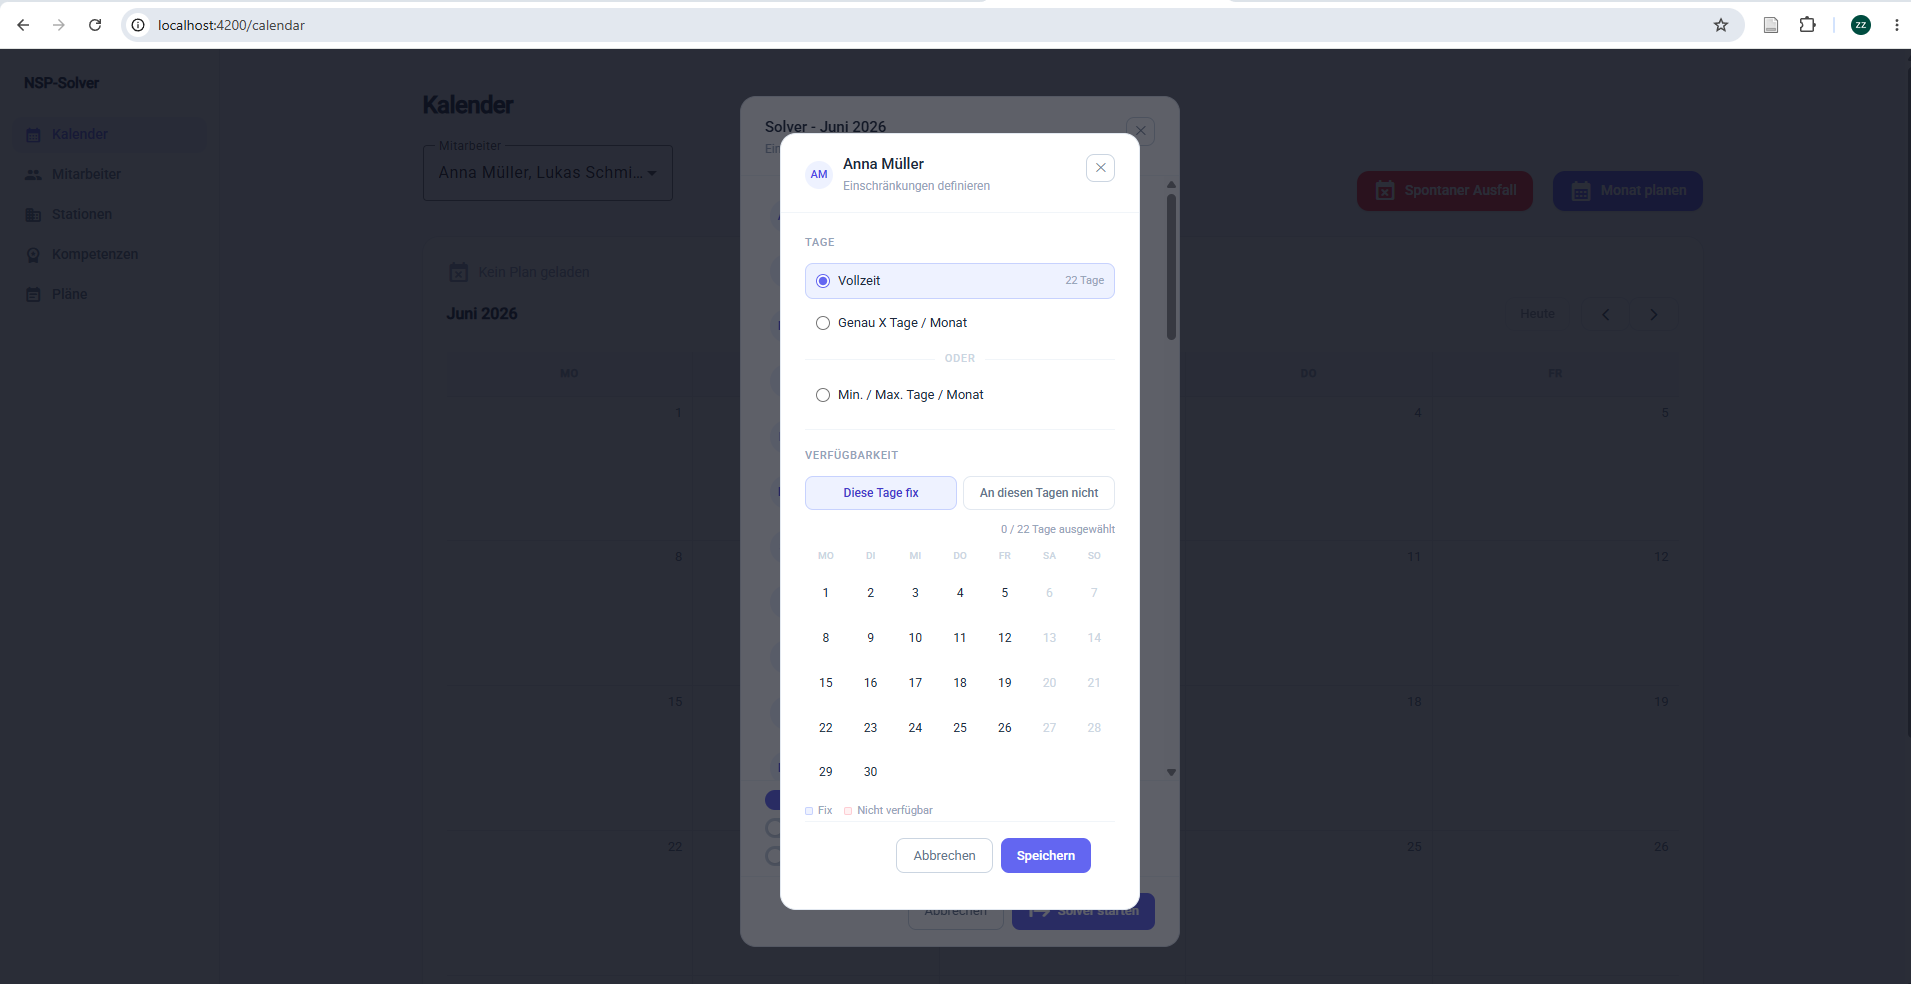
\includegraphics[width=\linewidth]{figures/constraint_dialog}
	\caption{
		Einschränkungs-Dialogfenster
	}\label{fig:constraint_dialog}
\end{figure}

Nach erfolgreichem Planungslauf werden die Zuteilungen direkt im Kalender angezeigt. Wie in Abbildung \ref{fig:calendar_full} ersichtlich, erscheinen pro Tag die zugeteilten Mitarbeiter als farbige Chips im jeweiligen Kalenderfeld.

\begin{figure}[H]
	\centering
	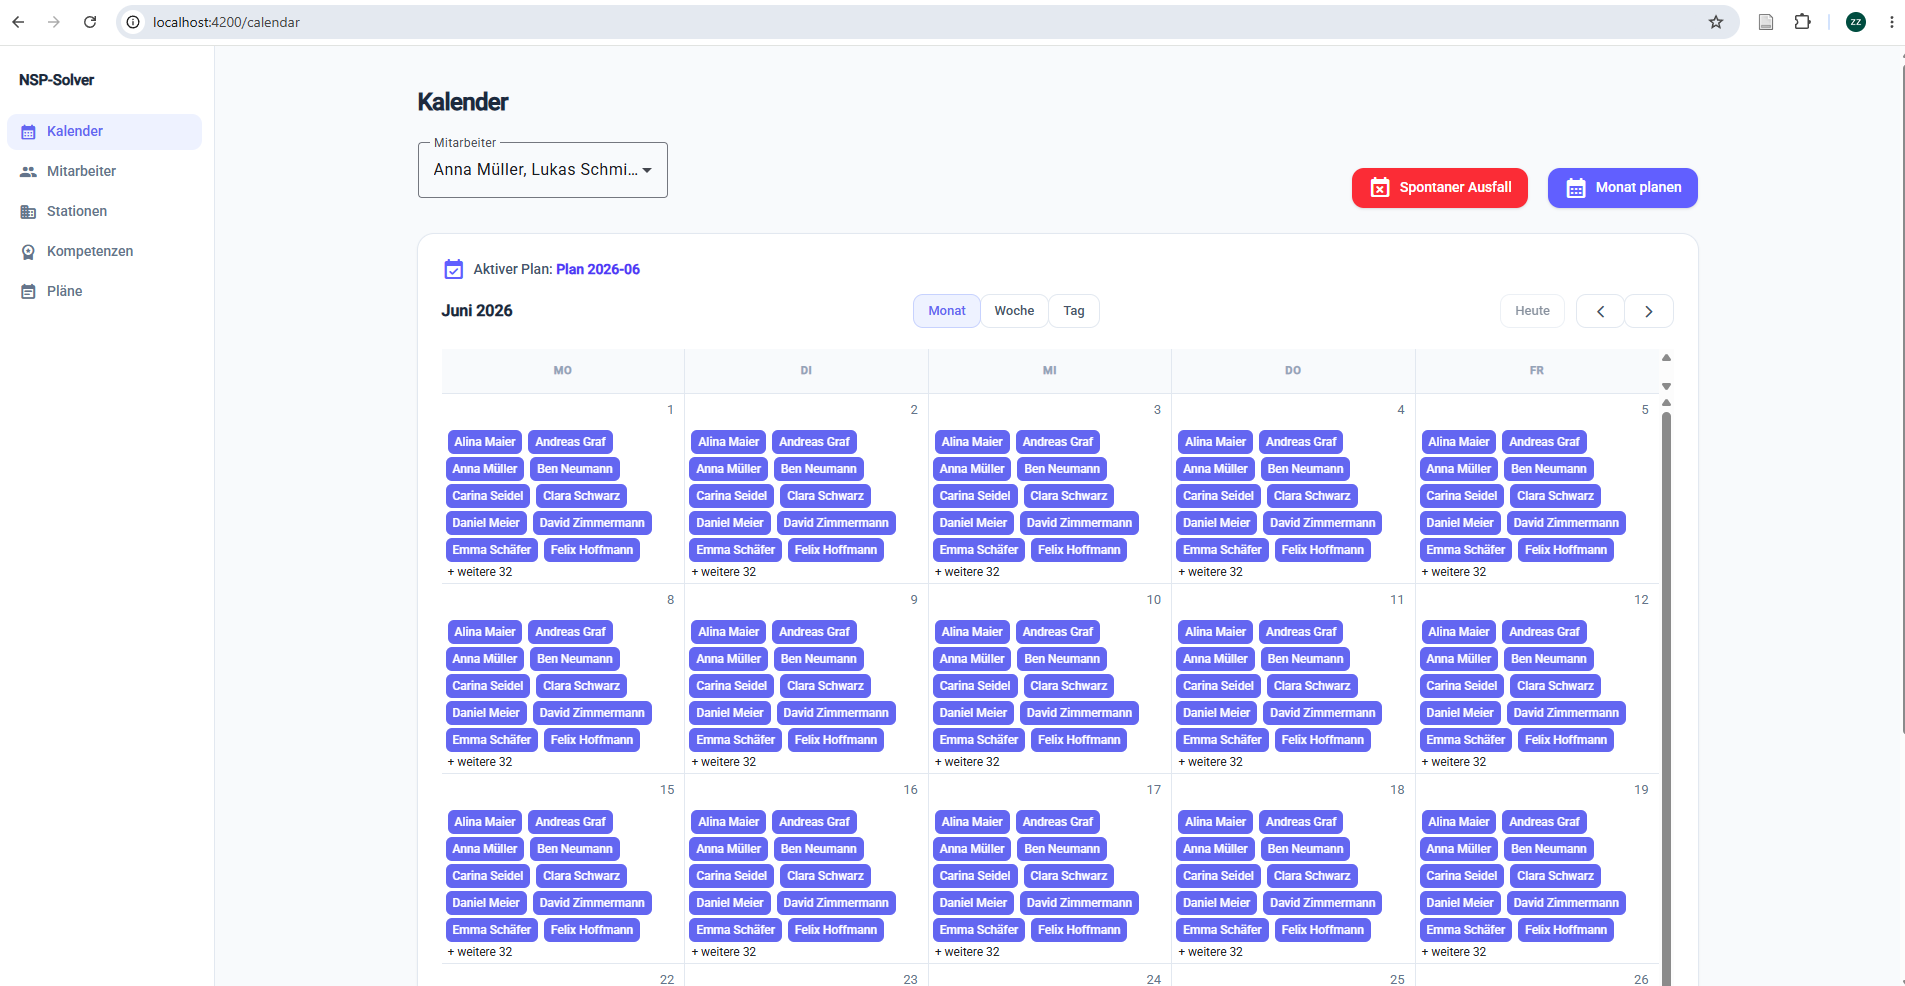
\includegraphics[width=\linewidth]{figures/calendar_full}
	\caption{
		Monatsübersicht mit Zuteilungen
	}\label{fig:calendar_full}
\end{figure}

 Über einen Klick auf einen beliebigen Tag gelangt man zur Tages-Detailansicht, in der, wie in Abbildung \ref{fig:day_detail} dargestellt, alle Stationen des jeweiligen Tages tabellarisch aufgelistet sind. Zu jeder Station ist der aktuelle Besetzungsstand sowie die namentliche Zuteilung der Mitarbeiter ersichtlich. Die Zuteilungen können dort bei Bedarf auch manuell über das Dropdown-Menü angepasst werden.
 
 \begin{figure}[H]
 	\centering
 	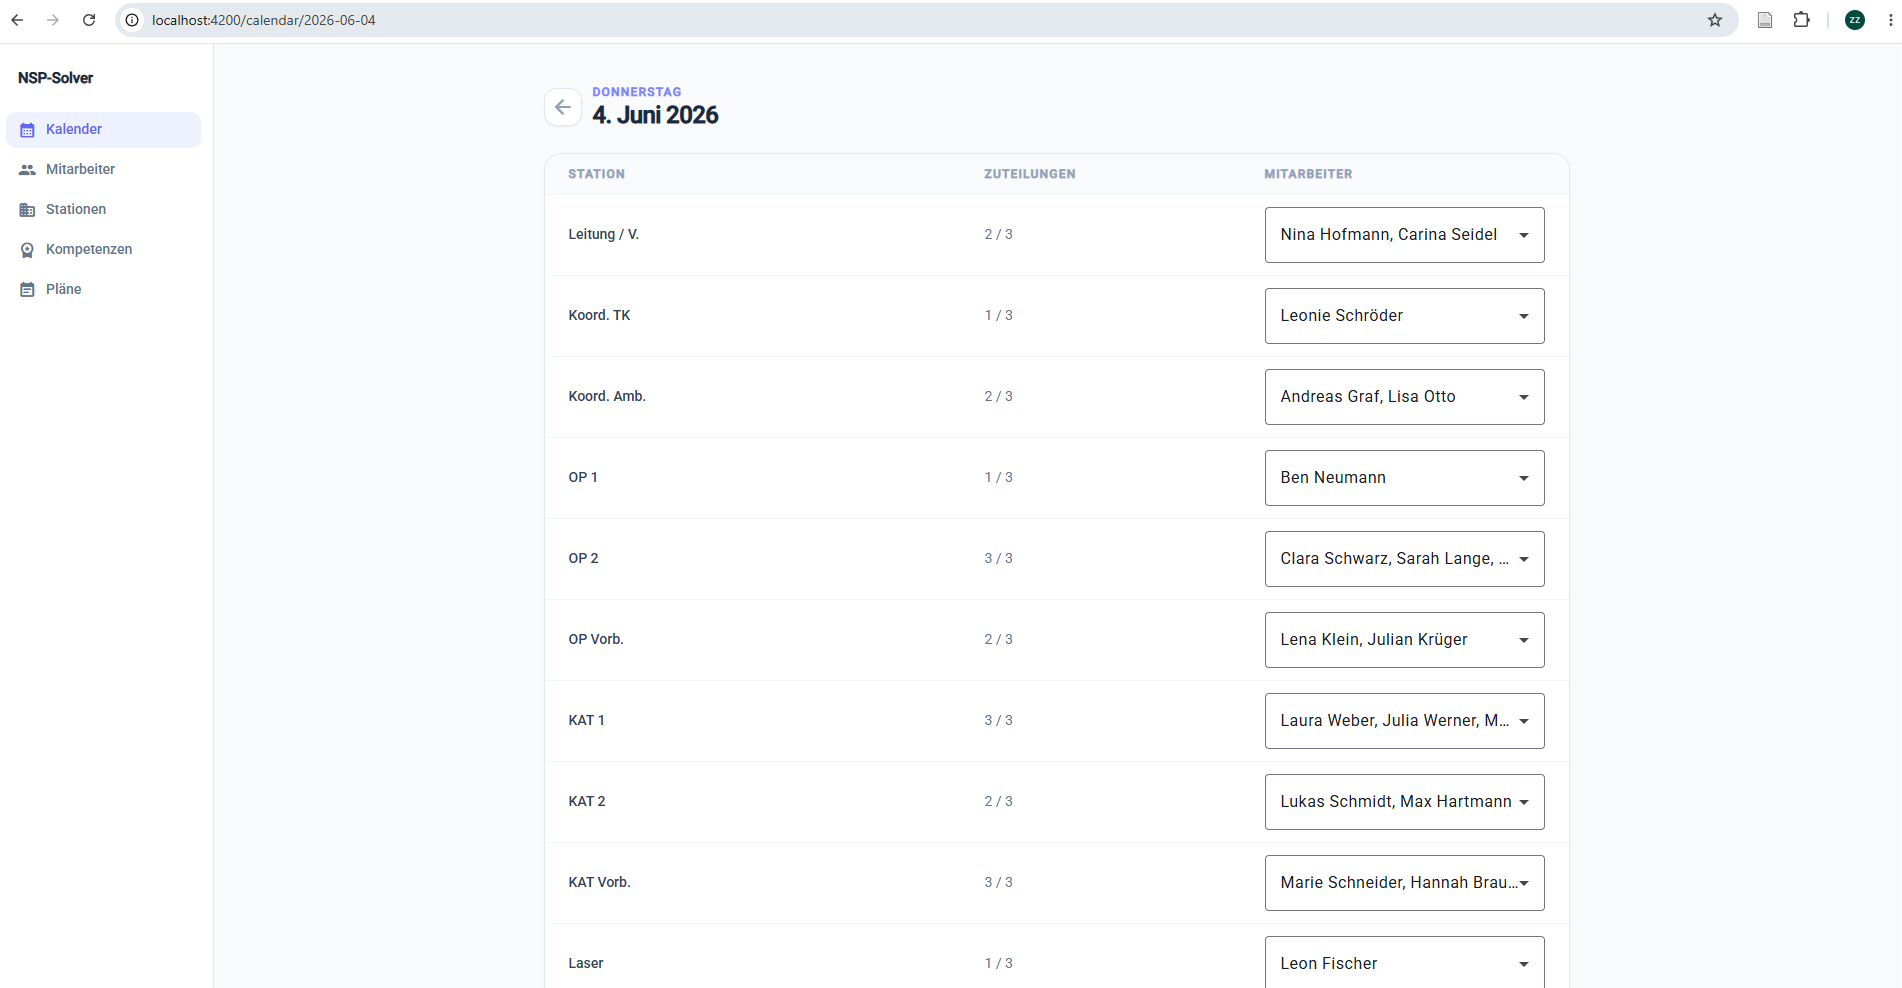
\includegraphics[width=\linewidth]{figures/day_detail}
 	\caption{
 		Monatsübersicht mit Zuteilungen
 	}\label{fig:day_detail}
 \end{figure}
 
 Fällt ein Mitarbeiter kurzfristig aus, kann über den Button \textit{Spontaner Ausfall} in der Kalenderansicht eine gezielte Umplanung ausgeführt werden. Wie in Abbildung \ref{fig:reschedule_dialog} ersichtlich, öffnet sich dabei ein Dialog, in dem für jeden Mitarbeiter ein Ausfall erfasst werden kann.
 
   \begin{figure}[H]
 	\centering
 	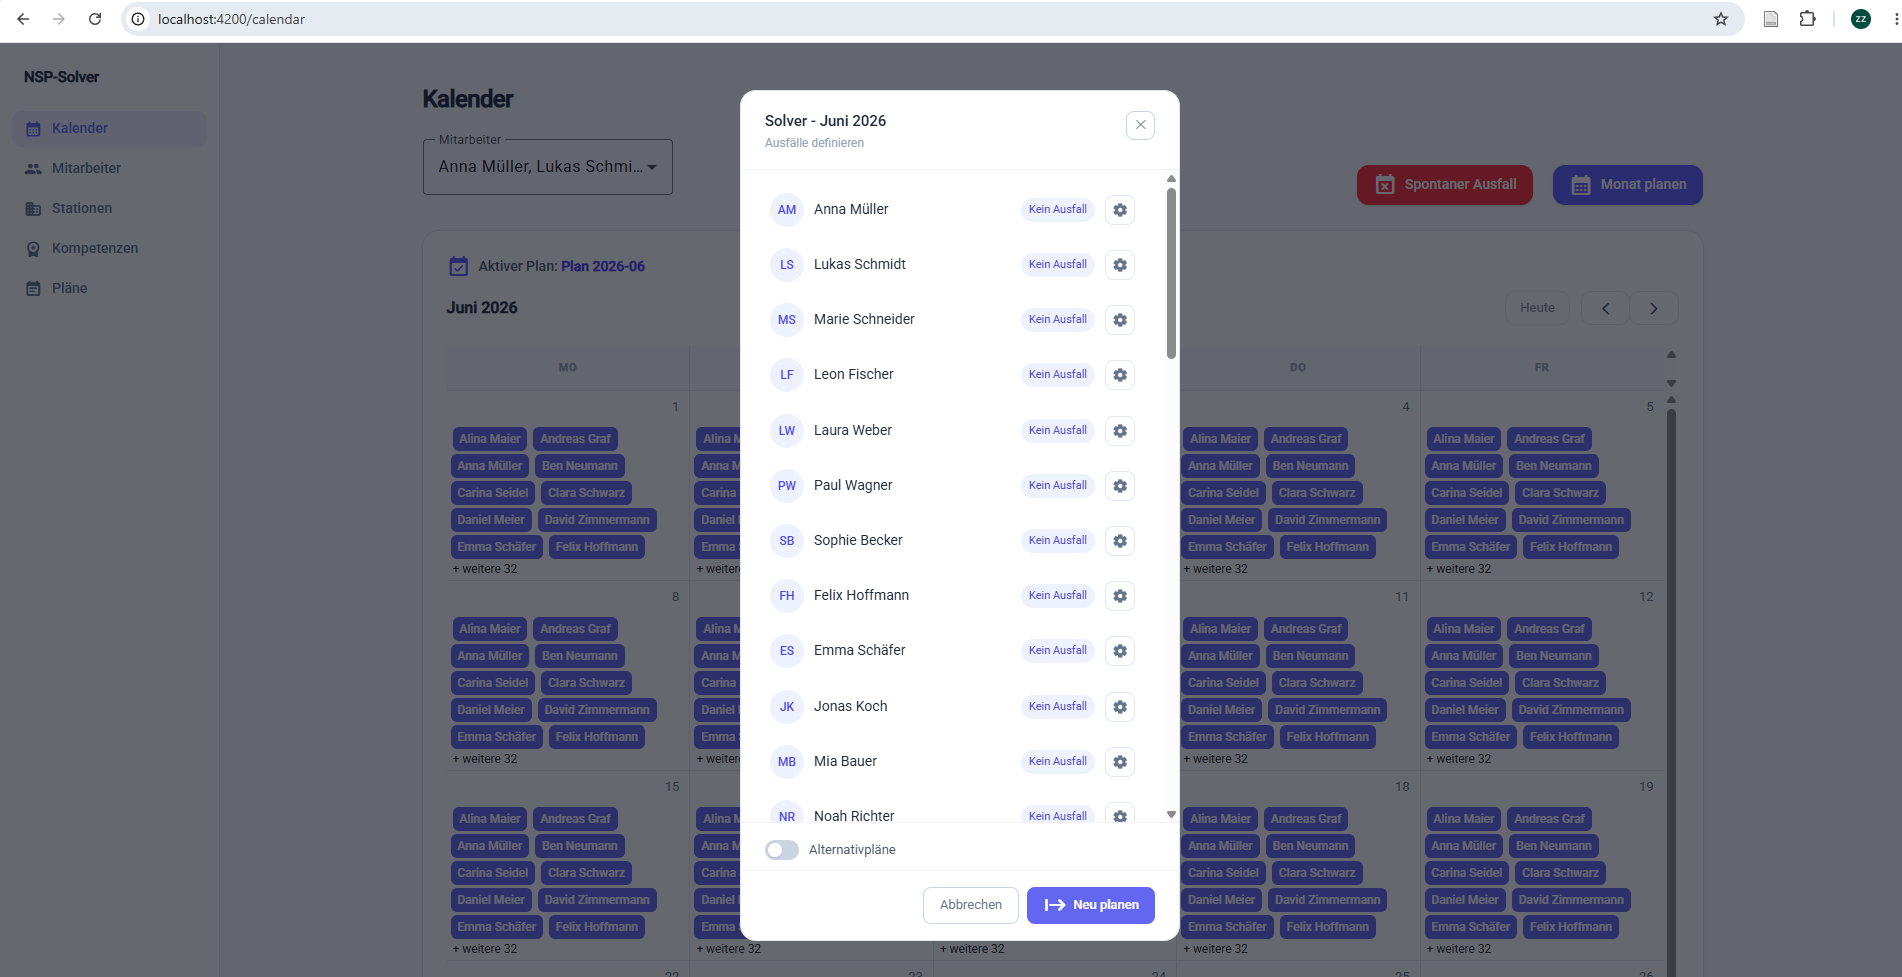
\includegraphics[width=\linewidth]{figures/reschedule_dialog}
 	\caption{
 		Reschedule-Dialogfenster
 	}\label{fig:reschedule_dialog}
 \end{figure}
 
  Per Klick auf das Zahnrad-Symbol neben einem Mitarbeiter lässt sich, wie in Abbildung \ref{fig:reschedule_constraint_dialog} dargestellt, ein Kalender öffnen, in dem die betroffenen Tage als nicht verfügbar markiert werden können. Optional kann über den Alternativpläne-Toggle gesteuert werden, ob zusätzliche Planvarianten generiert werden sollen. 
  
   \begin{figure}[H]
	\centering
	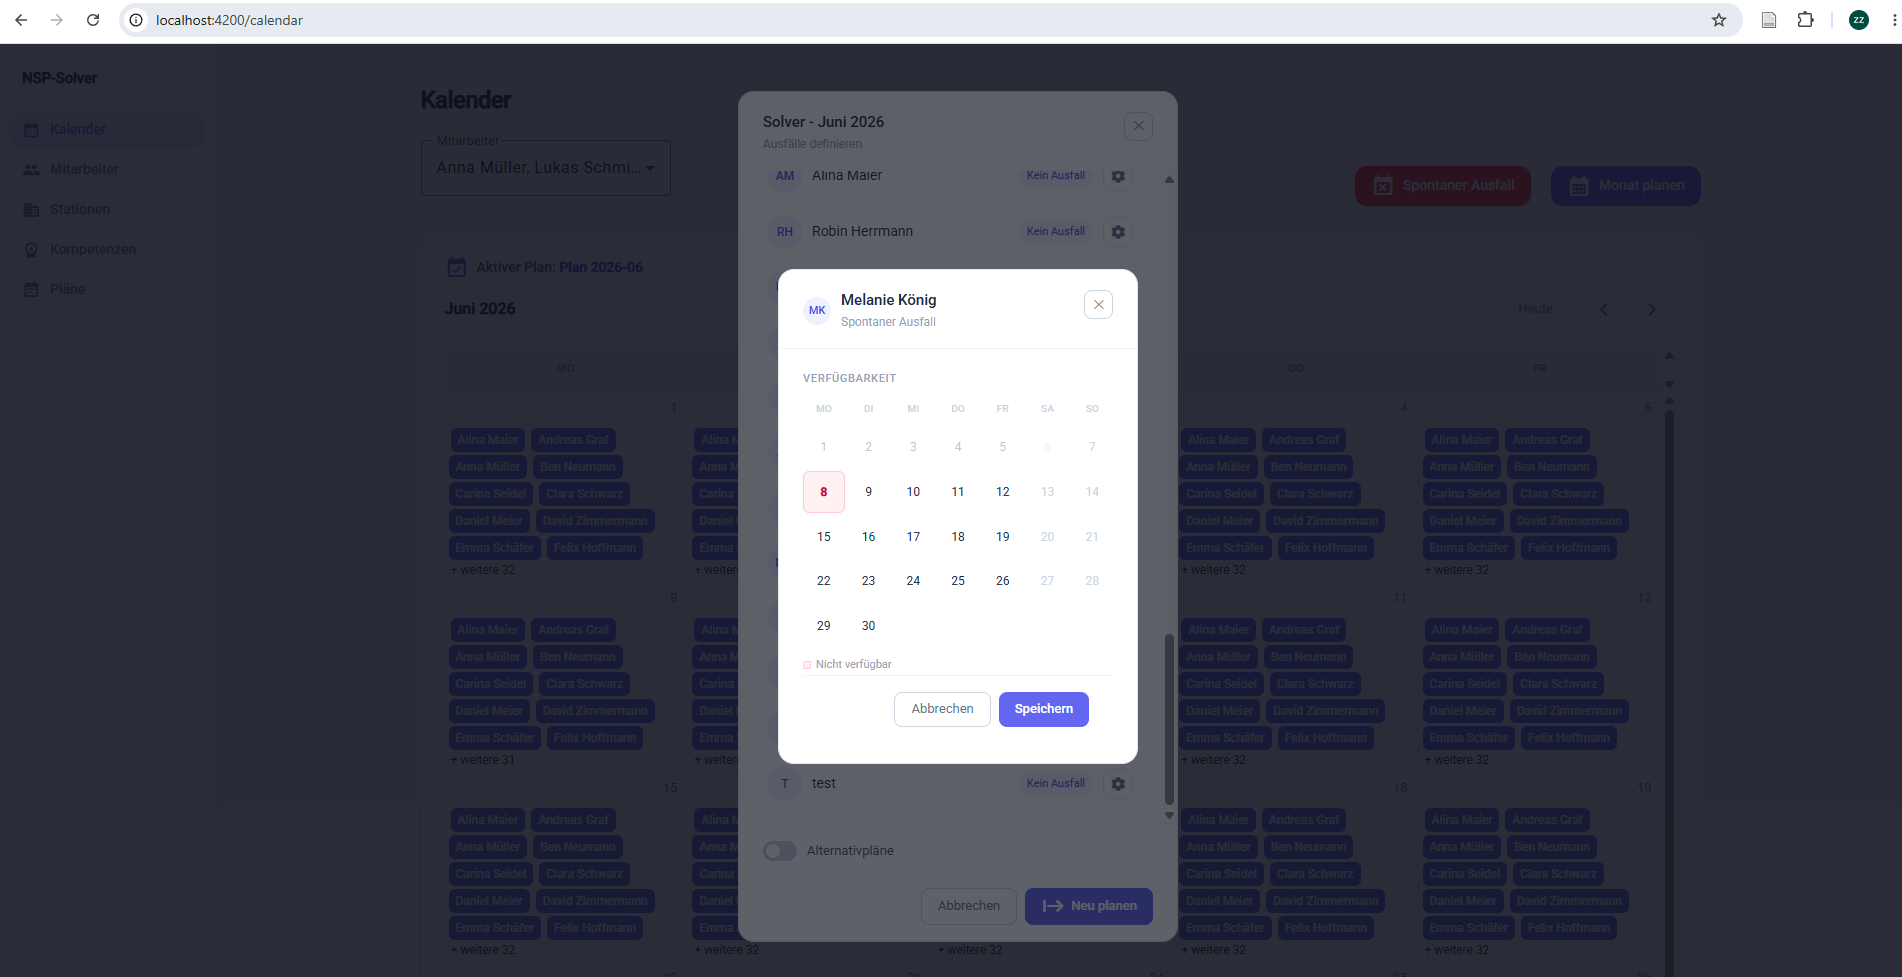
\includegraphics[width=\linewidth]{figures/reschedule_constraint_dialog}
	\caption{
		Reschedule-Dialogfenster - Einschränkungen
	}\label{fig:reschedule_constraint_dialog}
\end{figure}
  Nach dem Start der Umplanung mit \textit{Neu planen} aktualisiert der Solver den bestehenden Plan unter Berücksichtigung der neu definierten Ausfälle. Das Ergebnis wird anschließend in einem Zusammenfassungsdialog angezeigt, wie in Abbildung \ref{fig:reschedule_result} zu sehen, der übersichtlich auflistet, welche Zuteilungen entfernt und welche neu hinzugefügt wurden.

   \begin{figure}[H]
 	\centering
 	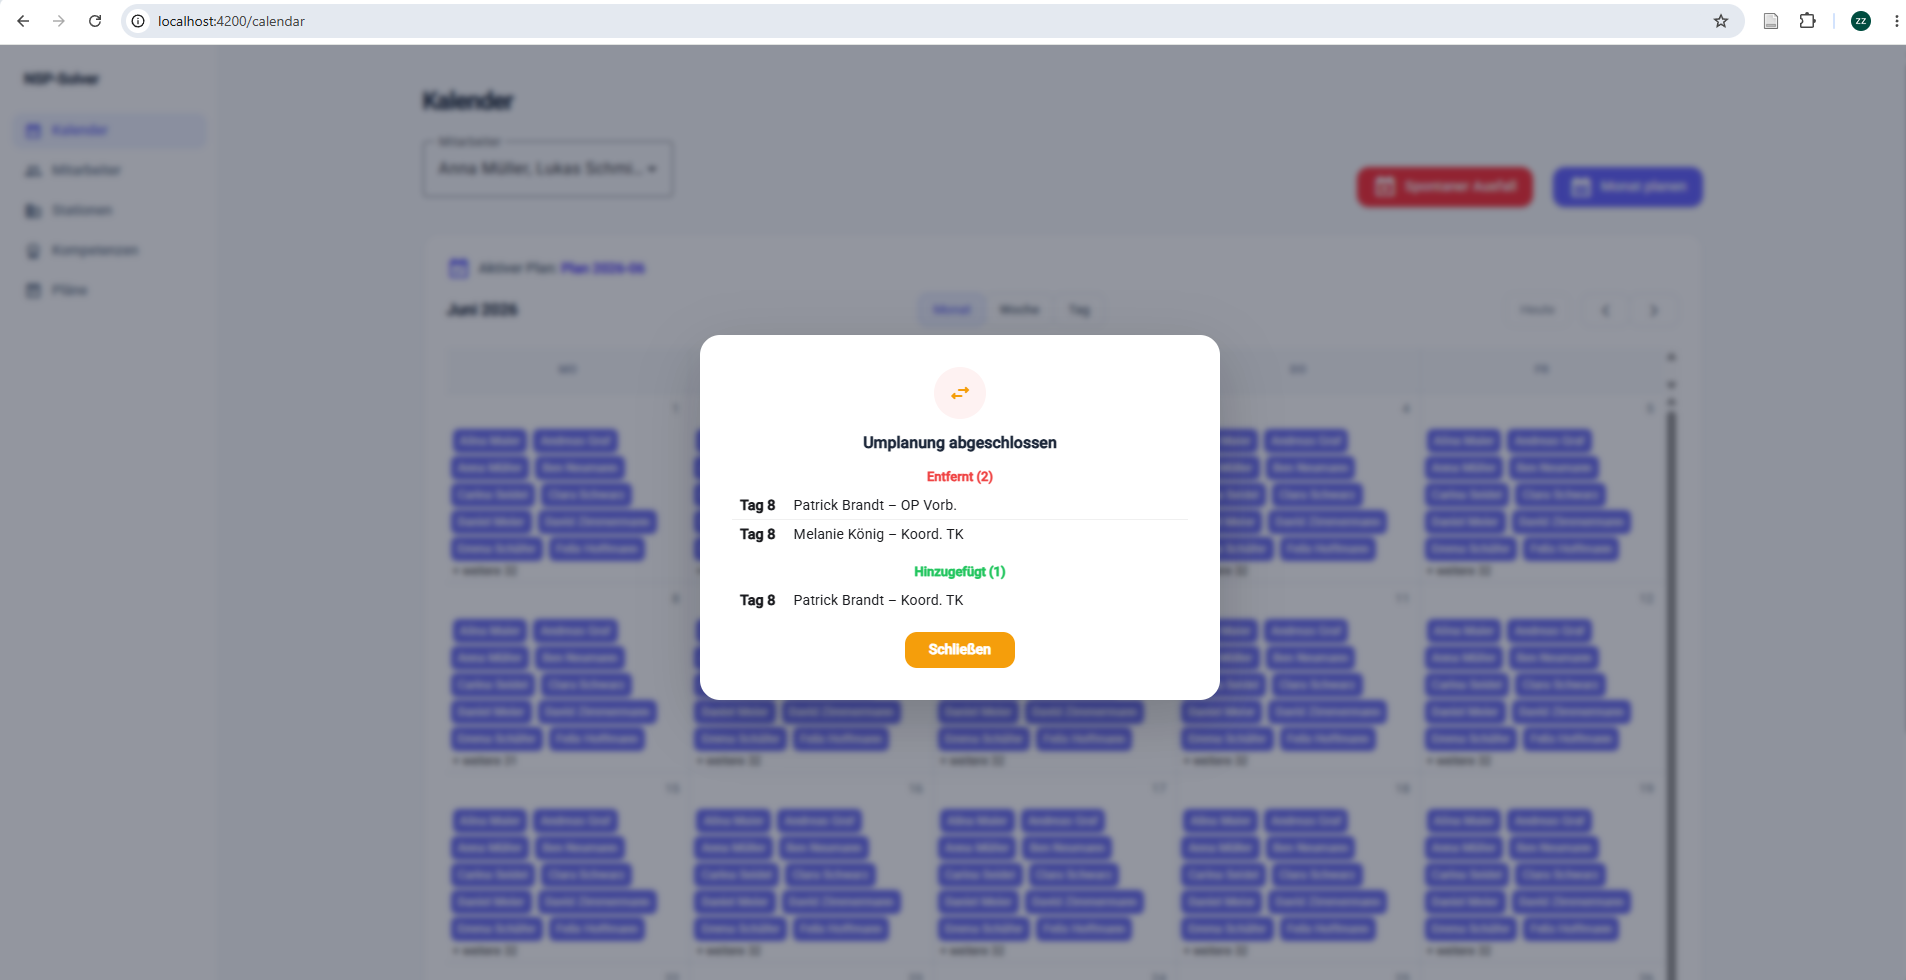
\includegraphics[width=\linewidth]{figures/reschedule_result}
 	\caption{
 		Reschedule-Ergebnis
 	}\label{fig:reschedule_result}
 \end{figure}
 
 




